% Provenance (never printed): cycle 2 "Questionner l'espace et le temps"
% (oceans, seas, continents on the globe) and "Questionner le monde de la
% matiere" (states of water in natural phenomena); see sources/book1/PROVENANCE.md.
% Book 1, grade 2, chapter 1.
\chapter{Water op Aarde}\label{ch:g2:water-on-earth}

Op 7 december 1972 draaiden drie astronauten op weg naar de Maan hun
camera terug naar de Aarde. Hun foto werd een van de beroemdste foto's die
ooit zijn gemaakt. Kijk er maar eens naar. Je ziet witte wolken, een beetje
bruin en geel land, het witte ijs onderaan --- en blauw, overal blauw.
Vanuit de ruimte gezien is onze planeet een blauwe planeet.

\begin{omfigure}
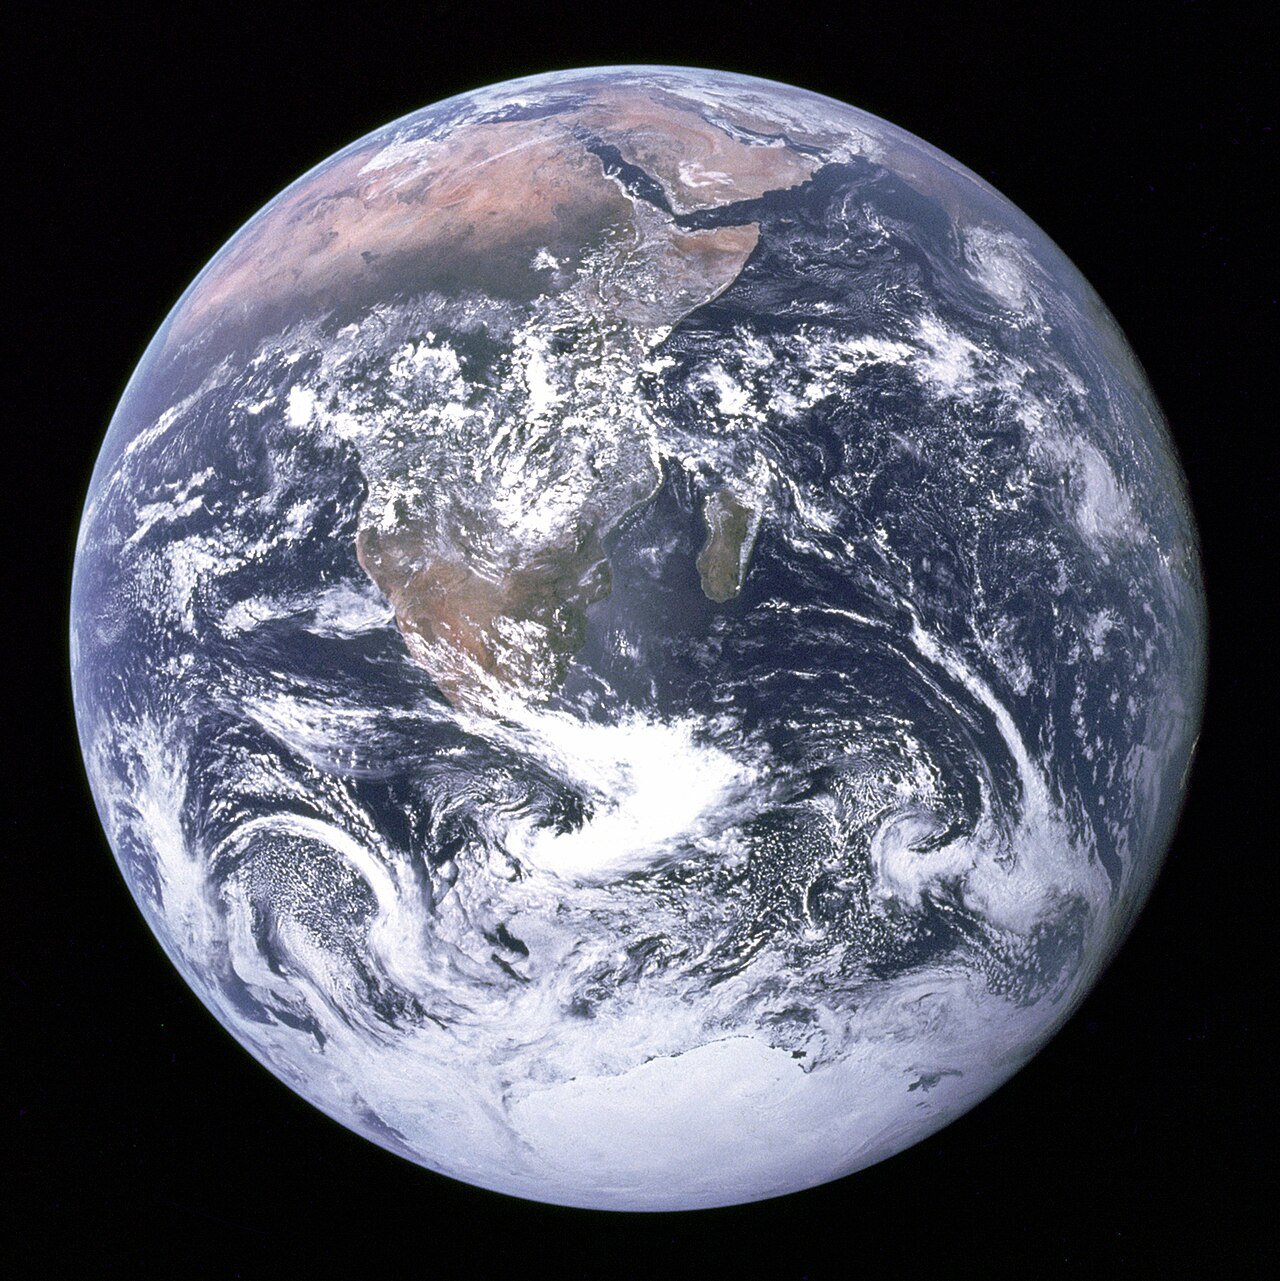
\includegraphics[width=0.5\linewidth]{images/book1/g2-nasa-blue-marble.jpg}

{\small De Aarde, gefotografeerd door de bemanning van Apollo~17,
7~december 1972. We zien Afrika, Arabië bovenaan en het ijs van
Antarctica onderaan. Foto: NASA (publiek domein).}
\end{omfigure}

\begin{recall}
Water kan vast zijn (ijs), vloeibaar, of een gas dat we niet kunnen zien
(waterdamp). Vloeibaar water dat in de zon staat, wordt langzaam damp: het
verdampt. Als de damp afkoelt, wordt hij weer piepkleine druppeltjes: hij
condenseert. Deze veranderingen ken je uit de natuurkundeboeken. In een
\omterm{def:g1:landscapes-around-us:landscape}{landschap} stroomt water in \omterm{def:g1:landscapes-around-us:water}{rivieren} en ligt het in \omterm{def:g1:landscapes-around-us:water}{meren}
(\cref{ch:g1:landscapes-around-us}).
\end{recall}

\section{De blauwe planeet}

Het grootste deel van de Aarde is bedekt met water. Stel je voor dat we het
hele oppervlak van de Aarde in 100 gelijke vierkantjes verdelen. Als we elk
vierkantje dat door \omterm{def:g2:water-on-earth:ocean}{zee} bedekt is blauw kleuren, kleuren we er 71. Maar 29
vierkantjes zijn land.

\begin{omfigure}
\begin{tikzpicture}
  \begin{axis}[hide axis, width=7.2cm, height=7.2cm, xmin=-0.5, xmax=9.5,
      ymin=-0.5, ymax=9.5, axis equal image, scale only axis,
      clip=false]
    \addplot[scatter, only marks, mark=square*, mark size=9.2pt,
      scatter/classes={0={fill=green!45!omLithAlluv, draw=black!40},
                       1={fill=omSea!80!blue, draw=black!40}},
      point meta=explicit symbolic]
      table[x=col, y=row, meta=blue] {figdata/out/grade-2-ocean_fraction-grid.dat};
  \end{axis}
\end{tikzpicture}

{\small Als het oppervlak van de Aarde in 100 gelijke vierkantjes was
verdeeld, zouden er 71 \omterm{def:g2:water-on-earth:ocean}{zee} zijn (blauw) en 29 land (groen). Berekend uit
een kaart van het reliëf van de hele Aarde (NOAA ETOPO1).}
\label{fig:g2:water-on-earth:grid}
\end{omfigure}
% ledger: data:etopo1, wss:ocean-cover (71 % computed in figdata/grade-2/ocean_fraction.py)

De grote watervlakten met \omterm{def:g2:water-on-earth:salt-fresh}{zout water} die het grootste deel van de Aarde
bedekken, hebben namen.

\begin{definition}[Oceaan en zee]\label{def:g2:water-on-earth:ocean}
Een \emph{oceaan}\index{oceaan} is een van de heel grote watervlakten met
\omterm{def:g2:water-on-earth:salt-fresh}{zout water} die het grootste deel van de Aarde bedekken en tussen de
continenten liggen. Een \emph{zee}\index{zee} is een kleinere watervlakte
met \omterm{def:g2:water-on-earth:salt-fresh}{zout water}, meestal aan de rand van een oceaan en voor een deel door
land omsloten.
\end{definition}

Alle \omterm{def:g2:water-on-earth:ocean}{oceanen} zijn met elkaar verbonden: een boot zou van elke \omterm{def:g2:water-on-earth:ocean}{oceaan} naar
elke andere kunnen varen zonder over land te gaan. Hun namen, en waar ze op
een globe liggen, vind je in \cref{ch:g3:continents-and-oceans}.

\begin{omfigure}
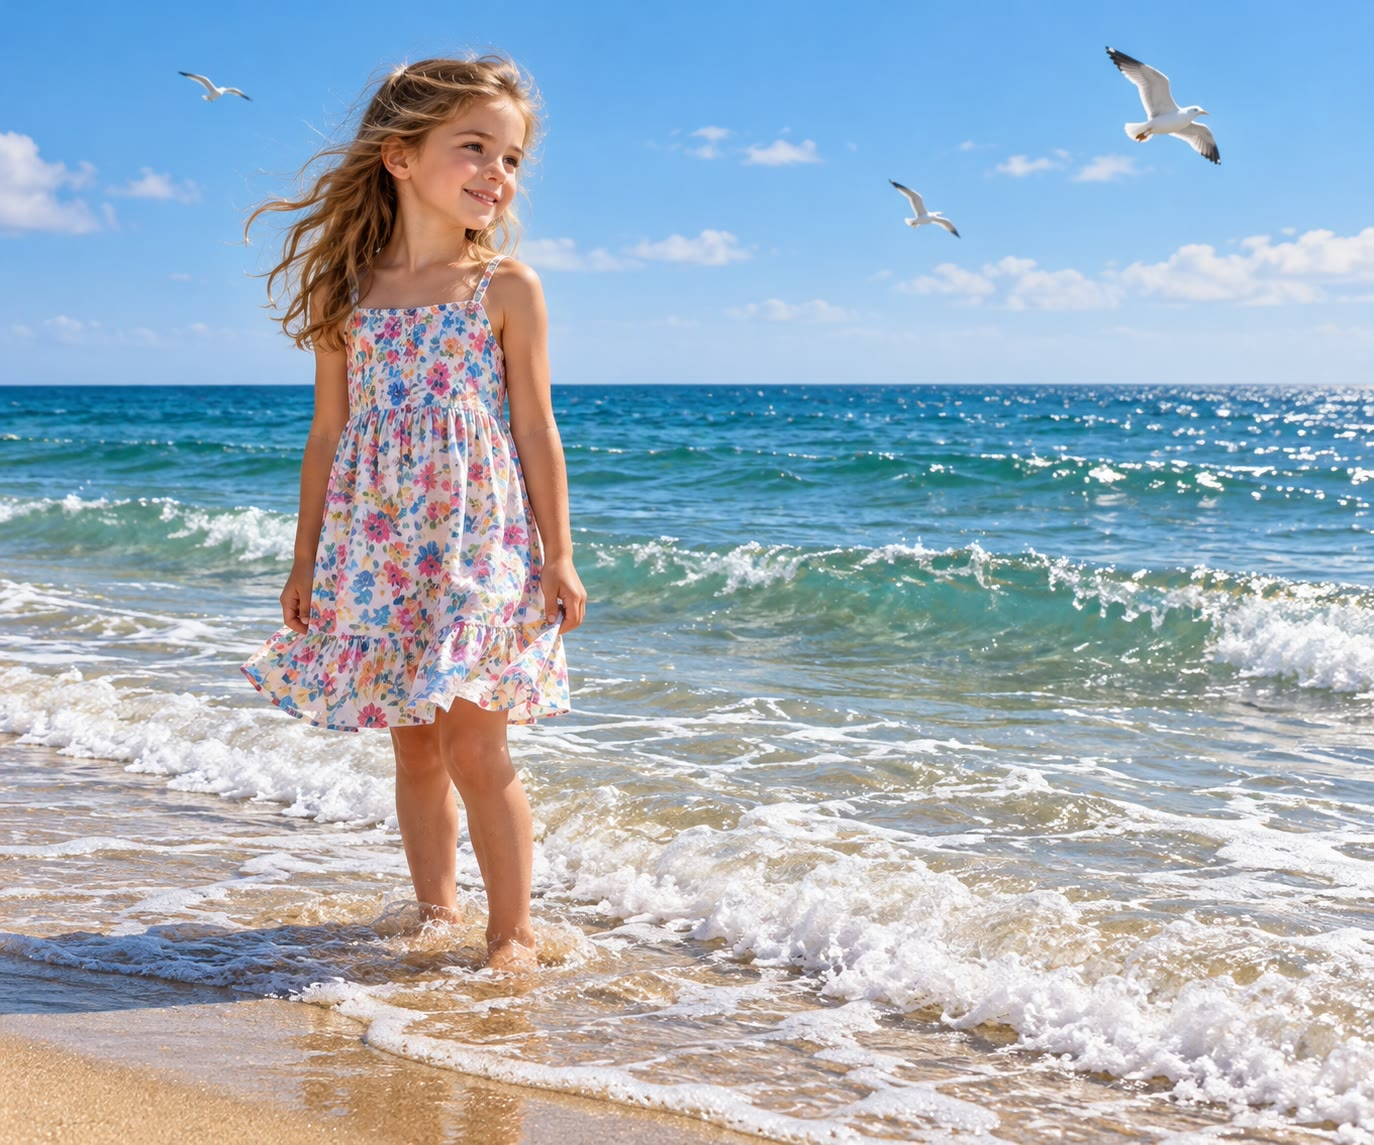
\includegraphics[width=0.62\linewidth]{images/book1/ai/g2-beach-sea.jpg}

{\small Aan de rand van de \omterm{def:g2:water-on-earth:ocean}{zee}. Het water gaat door, veel verder dan je
kunt kijken.}
\end{omfigure}

\section{Zout water en zoet water}

Heb je bij het zwemmen ooit een slok zeewater binnengekregen? Dan weet je
het: het smaakt heel zout. Het water van \omterm{def:g1:landscapes-around-us:water}{rivieren} en \omterm{def:g1:landscapes-around-us:water}{meren} niet.

\begin{definition}[Zout water en zoet water]\label{def:g2:water-on-earth:salt-fresh}
In \emph{zout water}\index{zout water} is veel zout opgelost: het is het
water van de \omterm{def:g2:water-on-earth:ocean}{oceanen} en de \omterm{def:g2:water-on-earth:ocean}{zeeën}. In \emph{zoet water}\index{zoet water}
zit heel weinig zout: het is het water van de regen, van de meeste \omterm{def:g1:landscapes-around-us:water}{rivieren}
en \omterm{def:g1:landscapes-around-us:water}{meren}, van het ijs en de sneeuw, en van bronnen.
\end{definition}

\begin{example}[Hoe zout is de zee?]\label{ex:g2:water-on-earth:salty}
% ledger: nos:salinity
In een fles met één kilogram zeewater --- ongeveer één liter --- zit
ongeveer 35 gram zout. Als we al het water laten verdampen, blijft het zout
als witte kristallen op de bodem achter. Zo wordt zeezout gemaakt in
zoutpannen aan \omterm{def:g2:water-on-earth:ocean}{zee}, waar de zon en de wind ondiepe plassen zeewater
langzaam laten opdrogen.
\end{example}

\begin{omfigure}
\begin{minipage}[b]{0.49\linewidth}\centering
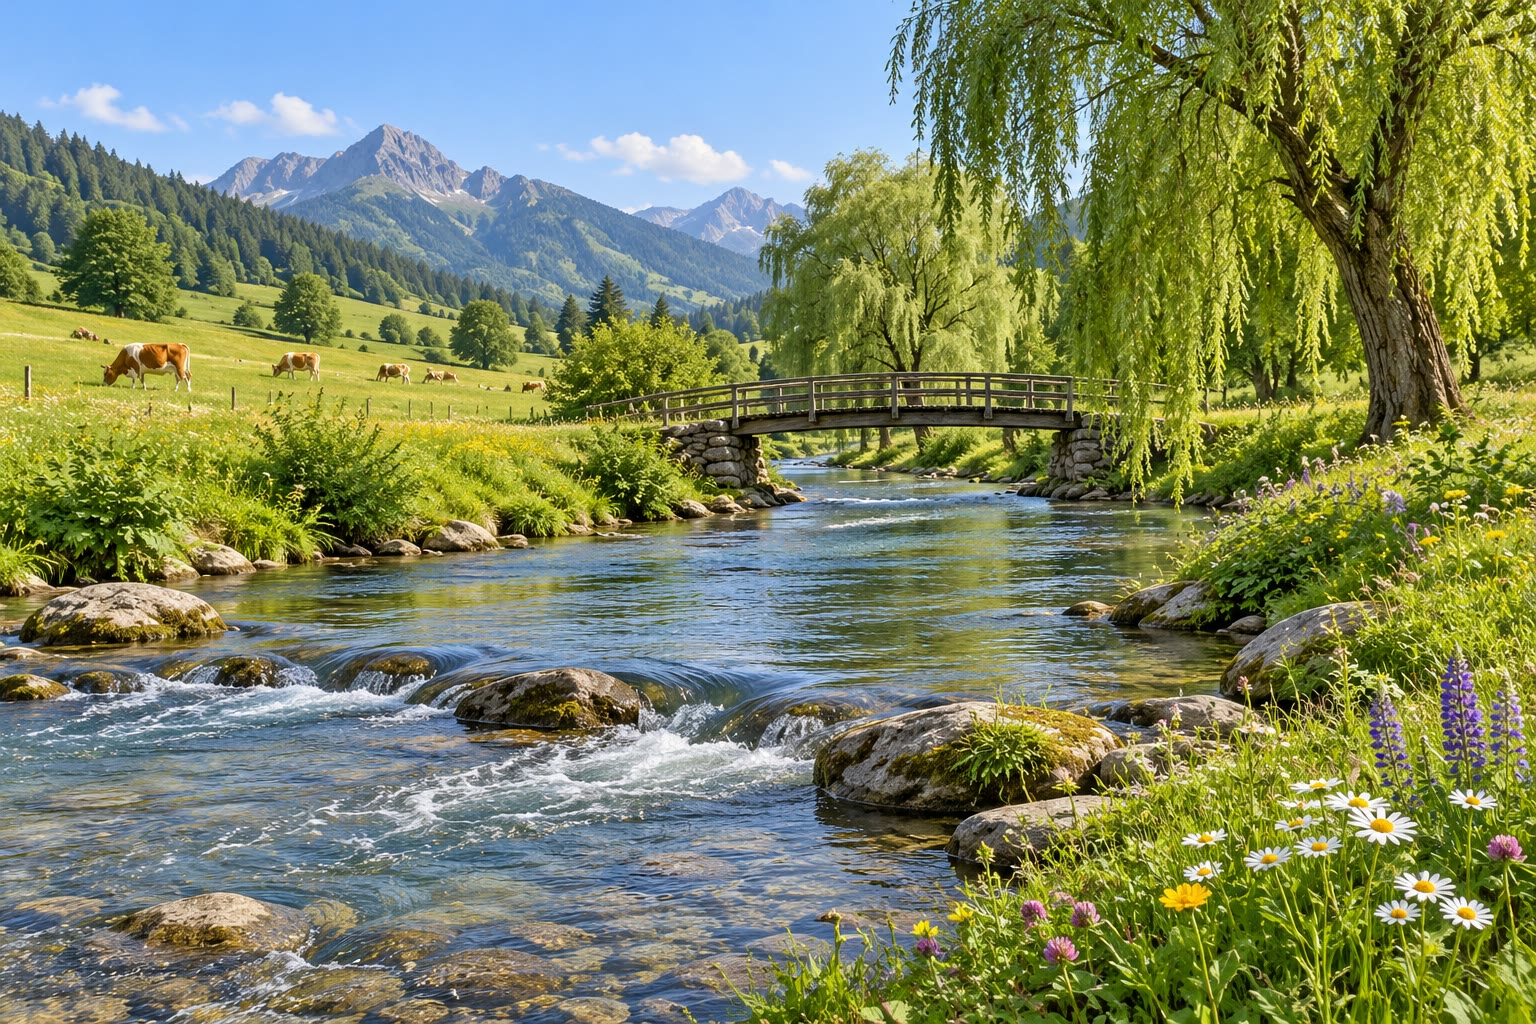
\includegraphics[width=\linewidth]{images/book1/ai/g2-river-meadow.jpg}

{\small \omterm{def:g2:water-on-earth:salt-fresh}{Zoet water}: een \omterm{def:g1:landscapes-around-us:water}{rivier}.}
\end{minipage}\hfill
\begin{minipage}[b]{0.49\linewidth}\centering
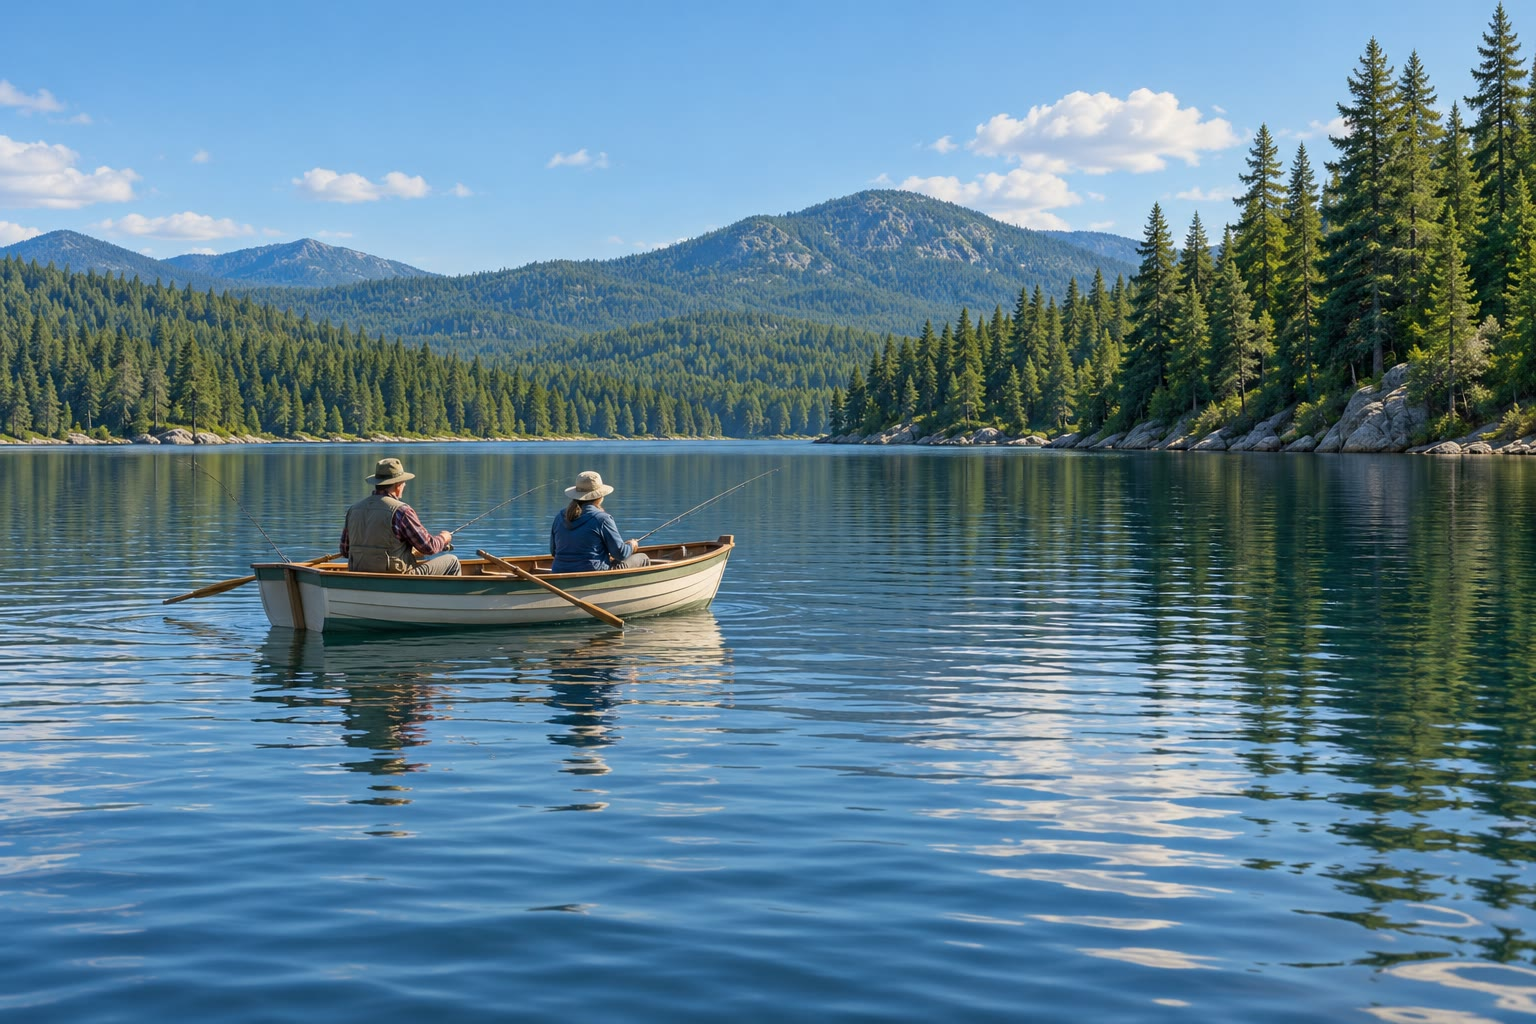
\includegraphics[width=\linewidth]{images/book1/ai/g2-lake-boat.jpg}

{\small \omterm{def:g2:water-on-earth:salt-fresh}{Zoet water}: een \omterm{def:g1:landscapes-around-us:water}{meer}.}
\end{minipage}
\end{omfigure}

\begin{remark}[Zeewater kun je niet drinken]\label{rem:g2:water-on-earth:drink}
Mensen en landdieren kunnen geen zeewater drinken: er zit te veel zout in,
en wie het drinkt, verliest juist water in plaats van het binnen te
krijgen. Zeelui ver op \omterm{def:g2:water-on-earth:ocean}{zee}, met overal water om zich heen, moesten daarom
altijd hun zoete water meenemen.
\end{remark}

\section{Waar is al het water?}

\omterm{def:g2:water-on-earth:salt-fresh}{Zoet water} zit niet alleen in \omterm{def:g1:landscapes-around-us:water}{rivieren} en \omterm{def:g1:landscapes-around-us:water}{meren}. Veel ervan is bevroren:
in het grote witte ijs van Antarctica en Groenland, en op de hoge \omterm{def:g1:landscapes-around-us:landform}{bergen}.
En veel ervan zit verborgen onder onze voeten, in de grond, waar het de
piepkleine ruimtes tussen zandkorrels en de spleten in het gesteente vult.

\begin{omfigure}
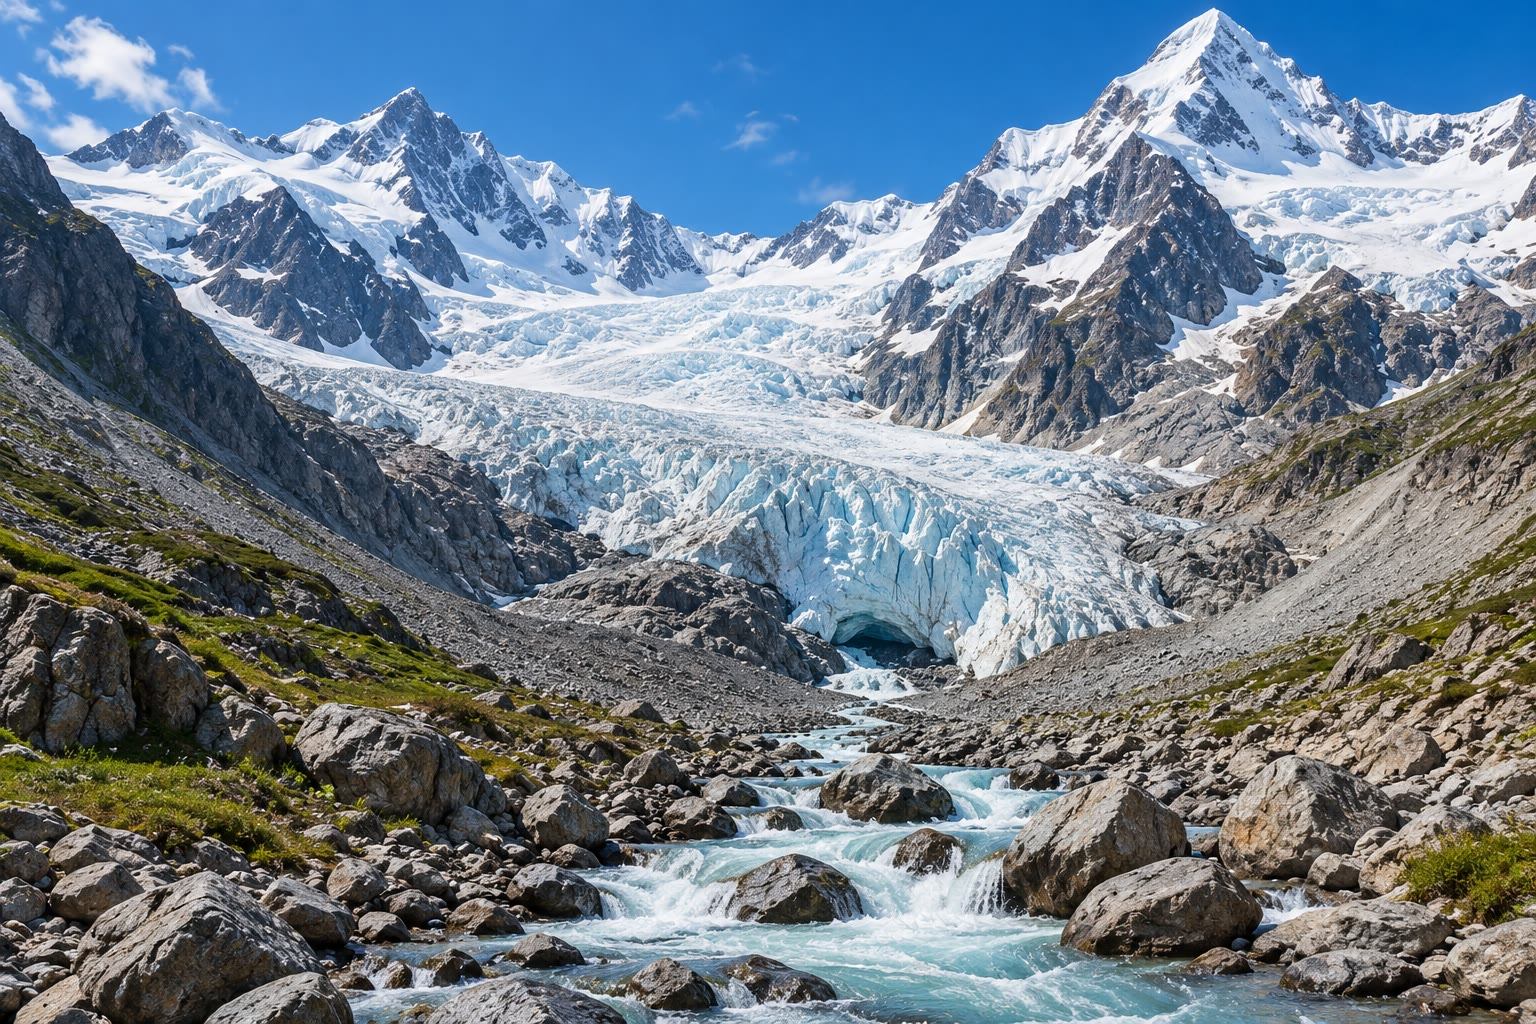
\includegraphics[width=0.62\linewidth]{images/book1/ai/g2-snowy-mountains.jpg}

{\small Hoge \omterm{def:g1:landscapes-around-us:landform}{bergen} bewaren het hele jaar \omterm{def:g2:water-on-earth:salt-fresh}{zoet water} als sneeuw en ijs. In
de zomer smelt er een deel van, dat de beken voedt.}
\end{omfigure}

Stel je voor dat we al het water van de Aarde in 100 even grote emmers
konden gieten. Hoeveel emmers zou elke soort water vullen?

\begin{omfigure}
\begin{tikzpicture}
  \begin{axis}[hide axis, width=7.2cm, height=7.2cm, xmin=-0.5, xmax=9.5,
      ymin=-0.5, ymax=9.5, axis equal image, scale only axis, clip=false]
    \addplot[scatter, only marks, mark=*, mark size=8pt,
      scatter/classes={0={fill=omSea!80!blue, draw=black!40},
                       1={fill=white, draw=black!60},
                       2={fill=brown!55, draw=black!40}},
      point meta=explicit symbolic]
      table[x=col, y=row, meta=kind] {figdata/out/grade-2-water_shares.dat};
  \end{axis}
  \begin{scope}[shift={(7.9,5.6)}, font=\small]
    \fill[omSea!80!blue, draw=black!40] (0,0) circle (0.2);
    \node[anchor=west] at (0.35,0) {zout water van de oceanen: 96 emmers};
    \fill[white, draw=black!60] (0,-0.7) circle (0.2);
    \node[anchor=west] at (0.35,-0.7) {ijs en sneeuw: 2 emmers};
    \fill[brown!55, draw=black!40] (0,-1.4) circle (0.2);
    \node[anchor=west] at (0.35,-1.4) {water onder de grond: 2 emmers};
  \end{scope}
\end{tikzpicture}

{\small Al het water van de Aarde in 100 emmers. De \omterm{def:g1:landscapes-around-us:water}{rivieren}, de \omterm{def:g1:landscapes-around-us:water}{meren}, de
wolken en het water van alle levende wezens samen zouden nog geen één
emmer vullen. Getallen van de U.S. Geological Survey.}
\label{fig:g2:water-on-earth:buckets}
\end{omfigure}
% ledger: wss:water-shares (rounded to 100 buckets in figdata/grade-2/water_shares.py)

\begin{proposition}[Het meeste water op Aarde is zout]\label{prop:g2:water-on-earth:most-salty}
% ledger: wss:water-shares
Van 100 emmers met al het water op Aarde zijn er 96 het zoute water van de
\omterm{def:g2:water-on-earth:ocean}{oceanen}. Het zoete water dat we drinken is maar een heel klein deel van al
het water: het meeste daarvan zit bevroren in het ijs, of verborgen onder
de grond.
\end{proposition}

\section{Waar gaat de regen heen?}

Als het regent, blijft het water niet liggen waar het valt. Kijk na een bui
maar eens naar het schoolplein: een deel van het water stroomt over de
grond naar de goten, een deel zakt in de aarde van de bloembedden, en
plassen verdwijnen langzaam als de zon weer gaat schijnen.

\begin{omfigure}
\begin{tikzpicture}[x=1cm, y=1cm, font=\small]
  % sky, sea, land
  \fill[ocBlue!6] (0,0) rectangle (12,5.6);
  \fill[omSea] (8.6,0) rectangle (12,0.9);
  \fill[green!30!omLithAlluv] (0,0) -- (0,2.4) .. controls (2,2.6) and (3,2.0) .. (4.5,1.6)
     .. controls (6,1.2) and (7.5,1.0) .. (8.6,0.9) -- (8.6,0) -- cycle;
  % ground below the surface
  \fill[brown!25] (0,0) rectangle (8.6,0.6);
  % river
  \draw[omSea!70!blue, line width=2.4pt] (1.6,2.45) .. controls (3.5,2.0) and (6,1.15) .. (8.6,0.95);
  % cloud and rain
  \pic at (2.2,4.0) {puffycloud};
  \foreach \x in {1.4,1.8,2.2,2.6,3.0}
    \draw[omWxRain, line width=0.8pt] (\x,3.7) -- (\x-0.15,3.1);
  \pic at (9.6,4.3) {puffycloud};
  % arrows
  \draw[omWxRain, line width=1.1pt, -{Stealth[length=2.5mm]}] (3.3,2.15) -- (3.3,0.6);
  \node[anchor=west, align=left, font=\scriptsize] at (3.4,1.0) {een deel zakt\\in de grond};
  \draw[omWxRain, line width=1.1pt, -{Stealth[length=2.5mm]}] (5.4,1.55) -- (7.6,1.15);
  \node[align=center, font=\scriptsize] at (6.2,2.05) {een deel stroomt naar een rivier,\\en de rivier stroomt naar zee};
  \draw[black!50, line width=1.1pt, densely dashed, -{Stealth[length=2.5mm]}] (10.2,1.1) .. controls (10.4,2.4) and (10.1,3.2) .. (9.8,3.85);
  \node[align=left, anchor=west, font=\scriptsize] at (10.45,2.4) {water\\verdampt};
  \draw[black!50, line width=1.1pt, densely dashed, -{Stealth[length=2.5mm]}] (8.45,4.35) -- (3.6,4.3);
  \node[font=\scriptsize, above] at (6.0,4.35) {de wind voert de wolken mee};
  \node[font=\scriptsize] at (10.4,0.45) {zee};
  \node[font=\scriptsize, anchor=west] at (0.2,3.25) {regen};
\end{tikzpicture}

{\small Waar de regen heen gaat. Het water dat als damp opstijgt uit de \omterm{def:g2:water-on-earth:ocean}{zee}
en van het land, vormt nieuwe wolken, en de wolken brengen nieuwe regen.}
\label{fig:g2:water-on-earth:rain}
\end{omfigure}

\begin{method}[Een regendruppel volgen]\label{met:g2:water-on-earth:drop}
Om een regendruppel te volgen, stel je drie vragen na elkaar:
\begin{enumerate}
  \item Waar valt hij: op de \omterm{def:g2:water-on-earth:ocean}{zee}, op een dak, op de grond, op een \omterm{def:g1:landscapes-around-us:landform}{berg}?
  \item Zakt hij in de grond, stroomt hij over het oppervlak weg, of
        bevriest hij tot ijs?
  \item Waar gaat hij daarna heen: naar een \omterm{def:g1:landscapes-around-us:water}{rivier}, een \omterm{def:g1:landscapes-around-us:water}{meer}, de \omterm{def:g2:water-on-earth:ocean}{zee}, de
        grond, of terug de lucht in?
\end{enumerate}
Uiteindelijk komt elke druppel terug in de \omterm{def:g2:water-on-earth:ocean}{zee} of in de lucht, en begint
de reis opnieuw.
\end{method}

\begin{example}[Een druppel op de berg]\label{ex:g2:water-on-earth:mountain}
Een regendruppel valt in de winter als sneeuw op een hoge \omterm{def:g1:landscapes-around-us:landform}{berg}. Hij blijft
daar bevroren liggen tot de warme dagen van de zomer. Dan smelt hij,
stroomt naar beneden in een bergbeek, komt in een \omterm{def:g1:landscapes-around-us:water}{rivier} terecht, en de
\omterm{def:g1:landscapes-around-us:water}{rivier} neemt hem mee naar \omterm{def:g2:water-on-earth:ocean}{zee}. Op een zonnige dag verdampt de druppel uit
de \omterm{def:g2:water-on-earth:ocean}{zee} en stijgt hij op in de lucht, waar hij deel wordt van een nieuwe
wolk.
\end{example}

\section{Oefeningen}

\begin{exercise}[$\star$]\label{exo:g2:water-on-earth:1}
\omterm{def:g2:water-on-earth:salt-fresh}{Zout water} of \omterm{def:g2:water-on-earth:salt-fresh}{zoet water}? De \omterm{def:g2:water-on-earth:ocean}{zee}; een \omterm{def:g1:landscapes-around-us:water}{rivier}; regen; een \omterm{def:g1:landscapes-around-us:water}{meer} in de
\omterm{def:g1:landscapes-around-us:landform}{bergen}; een \omterm{def:g2:water-on-earth:ocean}{oceaan}; het ijs op een \omterm{def:g1:landscapes-around-us:landform}{berg}.
\end{exercise}

\begin{exercise}[$\star$]\label{exo:g2:water-on-earth:2}
Waarom noemen we de Aarde de ``blauwe planeet''?
\end{exercise}

\begin{exercise}[$\star$]\label{exo:g2:water-on-earth:3}
In het rooster van 100 vierkantjes zijn er 71 blauw. Hoeveel vierkantjes
zijn land?
\end{exercise}

\begin{exercise}[$\star$]\label{exo:g2:water-on-earth:4}
Wat is groter, een \omterm{def:g2:water-on-earth:ocean}{oceaan} of een \omterm{def:g2:water-on-earth:ocean}{zee}?
\end{exercise}

\begin{exercise}[$\star$]\label{exo:g2:water-on-earth:5}
Kan een zeeman midden op de \omterm{def:g2:water-on-earth:ocean}{oceaan} het water rond zijn boot drinken?
Waarom?
\end{exercise}

\begin{exercise}[$\star$]\label{exo:g2:water-on-earth:6}
Noem drie plaatsen waar \omterm{def:g2:water-on-earth:salt-fresh}{zoet water} te vinden is.
\end{exercise}

\begin{exercise}[$\star\star$]\label{exo:g2:water-on-earth:7}
Hoeveel emmers zijn op het plaatje van de 100 emmers \omterm{def:g2:water-on-earth:salt-fresh}{zout water}? Hoeveel
zijn \omterm{def:g2:water-on-earth:salt-fresh}{zoet water} (ijs en water onder de grond samen)?
\end{exercise}

\begin{exercise}[$\star\star$]\label{exo:g2:water-on-earth:8}
Zet in volgorde, van wat het meeste water bevat naar wat het minste bevat:
de \omterm{def:g1:landscapes-around-us:water}{rivieren}; de \omterm{def:g2:water-on-earth:ocean}{oceanen}; het ijs en de sneeuw.
\end{exercise}

\begin{exercise}[$\star\star$]\label{exo:g2:water-on-earth:9}
Het regent op een akker. Noem twee dingen die met het water kunnen gebeuren.
\end{exercise}

\begin{exercise}[$\star\star$]\label{exo:g2:water-on-earth:10}
Een pan met zeewater blijft vele dagen in de zon staan, tot het water weg
is. Wat blijft er op de bodem van de pan achter? Waar is het water gebleven?
\end{exercise}

\begin{exercise}[$\star\star$]\label{exo:g2:water-on-earth:11}
Vertel de reis van een regendruppel die op het dak van de school valt, tot
hij weer in een wolk zit.
\end{exercise}
